\documentclass[10pt,a4paper,twocolumn]{article}
\usepackage[utf8]{inputenc}
\usepackage[francais]{babel}
\usepackage[T1]{fontenc}
\usepackage{amsmath}
\usepackage{amsfonts}
\usepackage{amssymb}
\usepackage{graphicx}
\title{Tiny Internet Project}
\author{Huysmans Guillaume,Lempereur Martin}
\begin{document}
\maketitle
\section{Introduction}
Le but de ce project était de reconstruire une certaine topologie composée de différents AS eux-même constitués de différents routeurs. En plus de cela nous devions paramétrer les routeurs pour que BGP fonctionne. Enfin nous devions configurer les filtres BGP pour que l'émission des routes respecte les différents liens commerciaux décrits dans l'énoncer et dont le comportement est défini dans le cours.
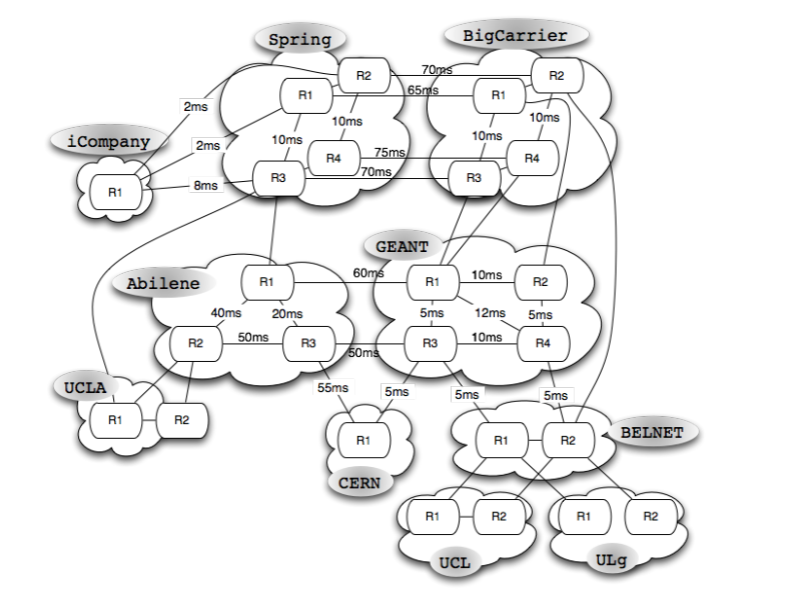
\includegraphics[scale=0.3]{topo.png}

\section{Création de la topologie}
En premier lieu nous avons créer l'ensemble des nœuds présents sur la topologie. Ensuite nous avons défini les AS par des numéros et avons ajouter chaque nœud à son numéro d'AS.
Après cela, il nous restait à créer les liens. Pour cela nous avons déterminé deux types de liens : les liens internes et les liens externes.
Les liens internes sont ceux qui sont présents au sein d'un même AS et permet à l'aide d'IGP qu'un routeur connaisse tout les autres routeur de son AS. Le deuxième type de liens a été utilisé lui pour connecter les routeurs de bordure entre eux et donc permettre l'échange de route BGP.

\section{Configuration des routeurs BGP}
Pour chaque routeur BGP donc qui se trouve en Bordure d'AS, on lui dit quel autre routeur BGP des autres AS est atteignable. De plus on explicite pour chaque routeur BGP quel sous-réseau il doit annoncer avec BGP. Après cela on dit que le routeur est actif.
\section{Filtres de routage}
Nous avons déterminé les différents liens commerciaux qu'ils existaient entre chaque AS. Une fois cela fait on a plus pour chaque routeur d'AS ajouter les filtres pour respecter le tableau suivant : 
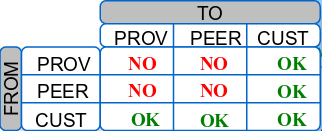
\includegraphics[scale=0.7]{comlink.png}
\section{Problèmes rencontrés}
Un soucis que nous n'avons pas pu corriger et que chaque routeur connait l'ensemble des routeurs présents dans son AS mais par contre, les routeurs de bordure n'arrivent pas a communiquer les routes BGP calculées à d'autres routeur que ceux qui ont un liens direct avec eux au seins de leur AS.
Par exemple dans notre cas R3 de Spring ne peux communiquer les routes BGP à R2 alors que R1 et R4 eux les connaissent. Alors que il existe une route IGP de R3 vers R2.
\section{Outils utilisés}
Pour nous simplifier l'écriture de notre script nous avons utilisé le système de macros proposé par m4.
Ainsi nous avons pu regrouper plusieurs commandes au seins d'une seule macros.
\end{document}